\chapter{Odoo Sous Docker}

	Dans ce qui suit, nous allons donner une idée sur l'interface que fournit Docker pour la provision des services (conteneurs). Nous allons réalisé la mini-architecture suivante:
	
	\begin{figure}[H]
	\centering
	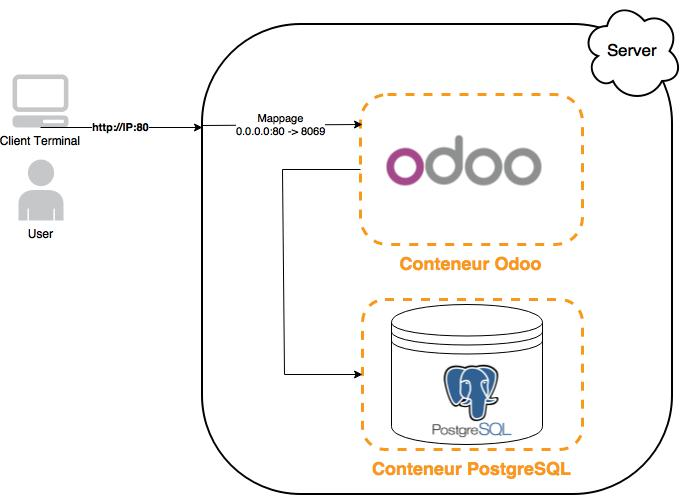
\includegraphics [scale=0.5]{biblio/odoo.jpg}
	\caption{Odoo sous Docker}
	\label{fig:}
	\end{figure}

\section*{Environnement technique}
	
	On va partir d'un serveur Ubuntu 14.04-64 bits avec Docker installé (L'installation ne sera pas détaillé), ou de préférence, un serveur CoreOS où Docker est déja inclut avec ce système d'éxploitation. A noter que Docker nécéssite un linux 64 bits avec un noyau >= 3.8.


\section*{Installation de PostgreSQL}

	Odoo a besoin d'un serveur de base de donnée PostgreSQL, la commande suivante permet de l'installer:

	\begin{lstlisting}[caption=Installation de PostgreSQL]
		$ docker run -d -e POSTGRES_USER=odoo -e POSTGRES_PASSWORD=odoo --name db postgres
	\end{lstlisting}




\section*{Installation d'Odoo}

	L'installation d'Odoo se fait grâce à la commande suivante:
	\begin{lstlisting}[language=bash,caption=Installation d'Odoo]
		$ docker run -p 80:8069 --name odoo --link db:db -t odoo
	\end{lstlisting}

	En quelques secondes, on pu lancer le service Odoo prêt à être utilisé, personnalisé, et éventuellement porté vers un autre serveur. Pour accéder au service il suffit de taper dans le navigateur:

	\begin{lstlisting}[language=bash]
		http://IP_SERVEUR:80
	\end{lstlisting}

	




\chapter{Docker-compose}

	On va réaliser l'installation détaillé dans \emph{l'Annexe A} avec l'outil \emph{Docker-compose}. Cet outil permet de définir dans un fichier YAML* l'architecture de l'application. Enfin, on peut faire des manipulation (démarrage, redémarrage, arrêt) sur toute l'architecture comme si c'était un seul service.

	\begin{lstlisting}[language=bash,caption=Installation d'Odoo avec Docker-compose]
		odoo:
	  		image: odoo
		  	links:
		   		- db
		  	ports:
		   		- "80:8069"
		db:
		  	image: postgres
		  	environment:
  				- POSTGRES_USER: odoo
  				- POSTGRES_PASSWORD: odoo
	\end{lstlisting}

	\begin{lstlisting}[language=bash,caption=Lancement d'Odoo avec Docker-compose]
		$ docker-compose up -d
	\end{lstlisting}